\subsubsection{Synthetic datasets}
A subset of the synthetic datasets used in this paper are used in both \cite{DBLP:conf/ida/MercierSASSS18} and \cite{santos2022joint}. These datasets were rebuild using the adapted dataset generator from \cite{santos2022joint} and dataset generator from \cite{DSPipe}. In addition we added the \emph{local imbalance} dataset as well as the \emph{uniform only boundary} dataset. The datasets \emph{02a} and \emph{02b} Figure \ref{fig:02a} and \ref{fig:02b} test the algorithms ability to predict groups within noise a noisy background distribution. Notice however that there are no noisy points within the subcluster distributions. The \emph{03subcl5} dataset Figure \ref{fig:03subcl5} tests 5 sub-clusters within a noisy background distribution in the same way as \emph{02a} and \emph{02b}, but the density of the clusters becomes smaller with the top one being the most dense, and the bottom one being the least dense. The \emph{clover} dataset Figure \ref{fig:clover} increases the size of the decision boundary, as well as testing the classifiers ability to handle a non gaussian distribution. The \emph{paw3} dataset shown in Figure~\ref{fig:paw3ob} tests the classifiers ability to predict borderline minority instances from a multi-modal minority distribution. The \emph{paw3} \emph{border dense center} is used in other papers, but tests the same problem as dataset \emph{02a} to the best of the authors knowledge.
The Gaussian overlap datasets are only shown for the case, where the means are respectively 1 and 4 standard deviations apart as shown in Figure \ref{fig:synthetic_dataset_gaussian_1} and \ref{fig:synthetic_dataset_gaussian_4}, but are evaluated with 2 and 3 standard deviations. 
\begin{figure}{}
    \centering
    \begin{subfigure}[t]{0.24\textwidth}
        \centering
        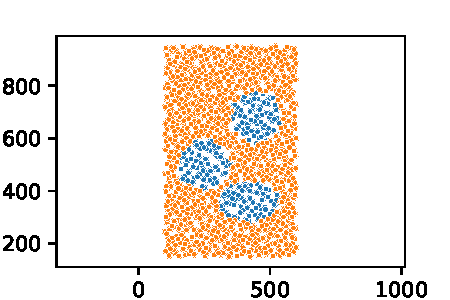
\includegraphics[width=\textwidth]{../plots/synthetic_dataset_visualizations/02a.csv.pdf}
        \caption[]%
        {{\small 02a}}    
        \label{fig:02a}
    \end{subfigure}
    \begin{subfigure}[t]{0.24\textwidth}  
        \centering 
        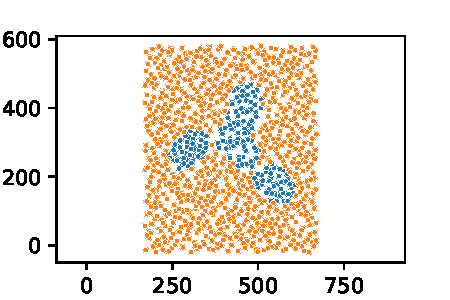
\includegraphics[width=\textwidth]{../plots/synthetic_dataset_visualizations/02b.csv.pdf}
        \caption[]%
        {{\small 02b}}    
        \label{fig:02b}
    \end{subfigure}
    \vskip\baselineskip
    \begin{subfigure}[t]{0.24\textwidth}  
        \centering 
        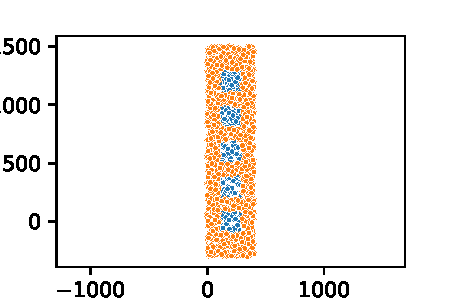
\includegraphics[width=\textwidth]{../plots/synthetic_dataset_visualizations/03subcl5.csv.pdf}
        \caption[]%
        {{\small 03subcl5}}    
        \label{fig:03subcl5}
    \end{subfigure}
    \begin{subfigure}[t]{0.24\textwidth}   
        \centering 
        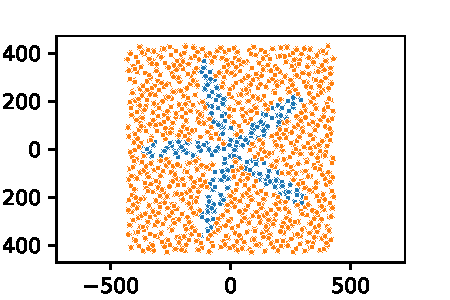
\includegraphics[width=\textwidth]{../plots/synthetic_dataset_visualizations/04clover5.csv.pdf}
        \caption[]%
        {{\small 04clover5}}    
        \label{fig:clover}
    \end{subfigure}
    \vskip\baselineskip
    \begin{subfigure}[b]{0.24\textwidth}   
        \centering 
        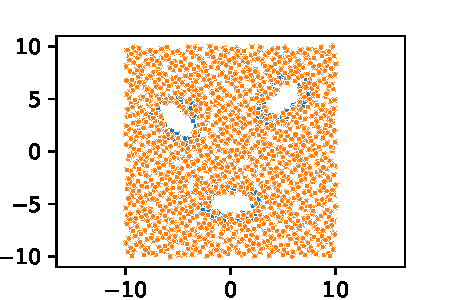
\includegraphics[width=\textwidth]{../plots/synthetic_dataset_visualizations/paw3-2d-only-border.csv.pdf}
        \caption[]%
        {{\small paw3 only border}}    
        \label{fig:paw3ob}
    \end{subfigure}
    \begin{subfigure}[b]{0.24\textwidth}   
        \centering 
        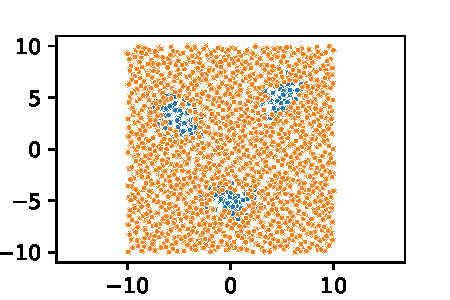
\includegraphics[width=\textwidth]{../plots/synthetic_dataset_visualizations/paw3-2d-border-dense-center.csv.pdf}
        \caption[]%
        {{\small paw3 border dense center}}    
        \label{fig:paw3bdc}
    \end{subfigure}
    \begin{subfigure}[b]{0.24\textwidth}
        \centering
        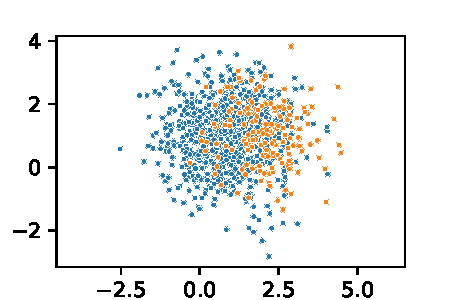
\includegraphics[width=\textwidth]{../plots/synthetic_dataset_visualizations/gaussian_overlap_0.83_0.17_1000_1_1.csv.pdf}
        \caption[Network2]%
        {{\small Gaussian overlap 1 standard deviations apart.}}    
        \label{fig:synthetic_dataset_gaussian_1}
    \end{subfigure}
    \hfill
    \begin{subfigure}[b]{0.24\textwidth}  
        \centering 
        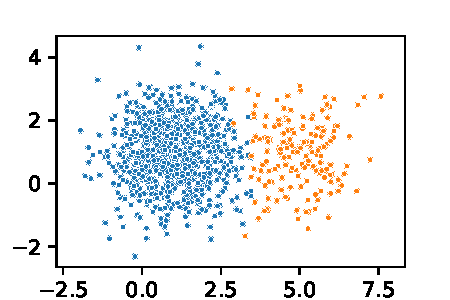
\includegraphics[width=\textwidth]{../plots/synthetic_dataset_visualizations/gaussian_overlap_0.83_0.17_1000_1_4.csv.pdf}
        \caption[]%
        {{\small Gaussian overlap 4 standard deviations apart.}}    
        \label{fig:synthetic_dataset_gaussian_4}
    \end{subfigure}
    \caption[]{\label{fig:synthetic-datasets-one} A subset of the synthetic datasets used in the experimental evaluation.}
\end{figure}
Overlap  comes in many forms as shown in \cite{santos2022joint} and one of the forms, that were not present in the existing dataset lineup was a local imbalance problem, where only a part of the dataset is in an overlapping region. This was created by making one uniform majority distribution, and two connected uniform minority distributions. The two uniform minority distributions have different densities to change the local imbalance degree. The overall imbalance ratio between minority and majority will however not be altered by a change in the local imbalance degree, as fewer points in the overlapping distribution, just results in more points in the non-overlapping distribution.
\begin{figure}
    \centering
    \vskip\baselineskip
    \begin{subfigure}[b]{0.24\textwidth}  
        \centering 
        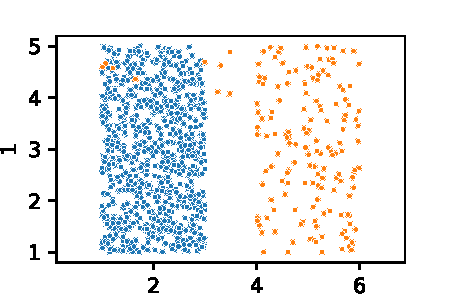
\includegraphics[width=\textwidth]{../plots/synthetic_dataset_visualizations/local_imbalance_degree_0.83_0.17_0.05_1000.csv.pdf}
        \caption[]%
        {{\small Local imbalance degree with an IR of 5, and 5 percent of the minority data in the local overlap region.}}    
        \label{fig:local_imbalance-degree_5_percent}
    \end{subfigure}
    \hfill
    \begin{subfigure}[b]{0.24\textwidth}   
        \centering 
        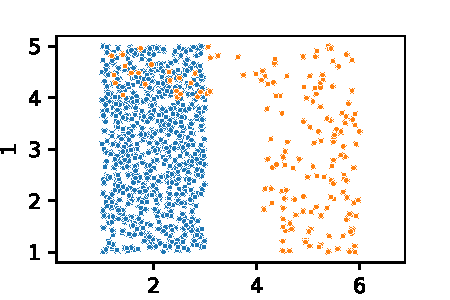
\includegraphics[width=\textwidth]{../plots/synthetic_dataset_visualizations/local_imbalance_degree_0.83_0.17_0.2_1000.csv.pdf}
        \caption[]%
        {{\small Local imbalance degree with an IR of 5, and 20 percent of the minority data in the local overlap region.}}    
        \label{fig:local_imbalance-degree_20_percent}
    \end{subfigure}
    \vskip\baselineskip
    \begin{subfigure}[b]{0.24\textwidth}   
        \centering 
        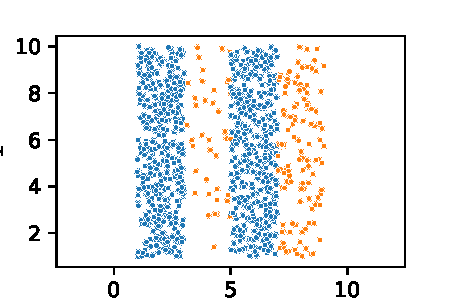
\includegraphics[width=\textwidth]{../plots/synthetic_dataset_visualizations/multi_modal_no_overlap_0.83_0.17_1000.csv.pdf}
        \caption[]%
        {{\small multi modal no overlap}}    
        \label{fig:multi_modal_no_overlap}
    \end{subfigure}
    \hfill
    \begin{subfigure}[b]{0.24\textwidth}   
        \centering 
        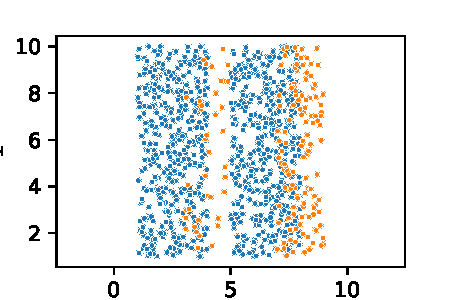
\includegraphics[width=\textwidth]{../plots/synthetic_dataset_visualizations/multi_modal_overlap_0.83_0.17_1000.csv.pdf}
        \caption[]%
        {{\small multi modal with overlap}}    
        \label{fig:multi_modal_with_overlap}
    \end{subfigure}
    \vskip\baselineskip
    \begin{subfigure}[b]{0.4\textwidth}   
        \centering 
        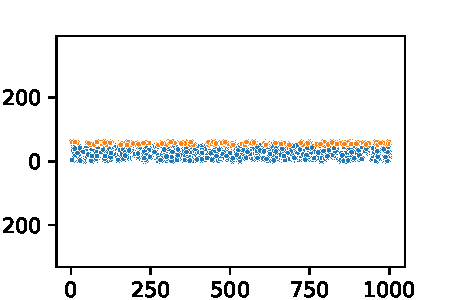
\includegraphics[width=\textwidth]{../plots/synthetic_dataset_visualizations/uniform_only_boundary_no_overlap_0.83_0.17_1000.csv.pdf}
        \caption[]%
        {{\small Uniform only boundary}}    
        \label{fig:uniform_only_boundary}
    \end{subfigure}
    \begin{subfigure}[b]{0.24\textwidth}
        \centering
        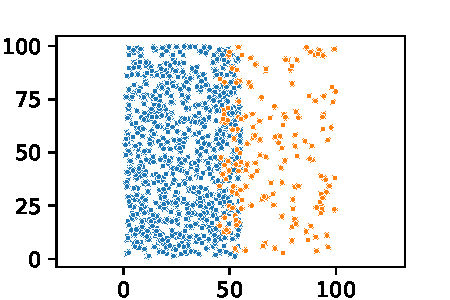
\includegraphics[width=\textwidth]{../plots/synthetic_dataset_visualizations/uniform_overlap_0.83_0.17_10_1000.csv.pdf}
        \caption[Network2]%
        {{\small 10\% overlap.}}    
        \label{fig:unform_overlap_10}
    \end{subfigure}
    \hfill
    \begin{subfigure}[b]{0.24\textwidth}  
        \centering 
        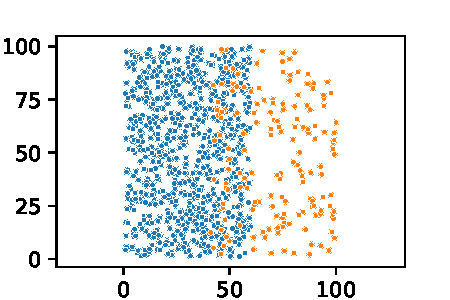
\includegraphics[width=\textwidth]{../plots/synthetic_dataset_visualizations/uniform_overlap_0.83_0.17_20_1000.csv.pdf}
        \caption[]%
        {{\small 20\% overlap.}}    
        \label{fig:uniform_overlap_20}
    \end{subfigure}
    \caption[]
    {\small A series synthetic datasets highlighting different overlap scenarios, and dataset complexities. The imbalance ratio in all of the illustrated datasets was $\text{IR}=5$.} 
    \label{fig:mean and std of nets}
\end{figure}


